\documentclass[a4paper, 12pt, twoside]{article}
\usepackage{ae,aecompl}
\usepackage[T1]{fontenc}
\usepackage[utf8]{inputenc}
\usepackage[ngerman]{babel}
\usepackage{textcomp}
\usepackage{anysize}
% left right up down
\marginsize{3.2cm}{2.8cm}{2cm}{2cm}
\usepackage{setspace}
\setstretch{1.2}
\frenchspacing
\usepackage{chemfig}
\usepackage{gensymb}
\usepackage{fancyhdr}
\usepackage{enumerate}
\usepackage{amsmath}
\usepackage{upgreek}
\usepackage{indentfirst}
\usepackage{sidecap}
\numberwithin{equation}{section}
\numberwithin{figure}{section}
\numberwithin{table}{section}
\usepackage{multicol}
\usepackage{float}
\setcounter{tocdepth}{1}
\pagestyle{empty}
% uncomment for hyperlinks
\usepackage{xcolor}
\usepackage[colorlinks = true,
            linkcolor = red,
            urlcolor  = blue,
            citecolor = blue,
            anchorcolor = blue]{hyperref}



\title{Laborpraxis für physikalische Chemie}
\author{\emph{verfasst von:} \\ Barna Kovács \\ Sándor Kunsági-Máté \\ András Kiss \\ Géza Nagy \\ \\ \emph{übersetzt von:} \\ András Kiss \\ \\ \\ \\ \\ \\

\includegraphics[width=0.2\textwidth]{fig/pte_logo.eps} \\
Abteilung für allgemeine und physikalische Chemie \\ Universität Pécs}

\begin{document}

\clearpage\maketitle
\thispagestyle{empty}
\newpage 
\tableofcontents
\newpage

%\setcounter{section}{1}
\section{Bestimmung des Dissoziationskonstante von schwachen Säuren mit Leitfähigkeitsmessung}
\subsection{Einleitung}

Elektrischer Widerstand ist eine Eigenschaft des Materials. Nach dem ohmschen Gesetz ist zwischen den Materialen durchpliessenden Stromstärke ($I$) und den Strom erstellenden Spannung ($U$) ein gerades Verhältniss.


\begin{equation}
\label{eq:ohm}
	U
	=
	I
	\cdot
	R
\end{equation}

wo der Verhältnissfaktor $R$ als Widerstand des Materials genannt wird, dessen Einheit ist der ohm ($\ohm$).
An spezifischer Widerstand verstehen wir den Quotient von der Spannung die zur Erstellung von ein 1 A starken Strom nötig ist und den Strom von 1 A. %%%

In der Elektrochemie ist es aus mehreren Hinsichten bevorzüglich, wenn wir den Reziprok von oben genannten Einheiten benutzen: den Reziprok vom Widerstand nenne wir Leitfähigkeit (Enheit ist Siemens, $S = 1 / \ohm$), den Reziprok von spezifischen Widerstand nenne wir spezifichen Leitfähigkeit (Einheit is $S/cm$).
An spezifischen Leitfähigkeit von Elektrolytlösungen ($\kappa$) nennen wir die Leitfähigkeit von Elektrolytlösung zwischen zwei Leitern von erste Klasse die 1 cm entfernt von einander sind und eine Fläche von 1 $cm^2$ haben.
Die spezifische Leitfähigkeit ist abhängig von der materilellen Qualität, von der Konzentration und von der Temperatur des Elektrolyten.
An molar spezifische Leitfähigkeit ($\Lambda _m$) verstehen wir den Quotient von der spezifischer Leitfähigkeit und der Konzentration.

\begin{equation}
\label{eq:lambdam}
        \Lambda_m
        =
        \frac
		{\kappa 1000 }
		{c}
	=
	\kappa V
\end{equation}

wo $c$ ist Konzentration (mol$\cdot$dm$^{-3}$), und $V$ ist Verdünnung.

Die molare Leitfähigkeit der unendlich verdünnten Lösüng wird molare Grenzleitfähigkeit genannt.
Nach Kohlrausch summiert sich die Leitfähigkeit von Anionen und Kationen in dünnen Lösungen von starken Elektrolyten. 

%Kohlrausch szerint erős elektrolitok híg oldataiban az anionok és kationok moláris fajlagos vezetőképessége összeadódik.

\begin{equation}
\label{eq:kohlrausch2}
	\Lambda _m^0
	=
	\lambda _a^0 \nu _a z_a + \lambda _k^0 \nu _k z_k
%	/1000
\end{equation}

wo $z_a, z_k$ sind die Ladung, $\nu _a, \nu _k$ sind die stöchiometrischen Faktoren, und $\lambda _a^0, \lambda _k^0$ sind die Grenzleitfähigkeiten von Anionen ($a$) und Kationen ($k$).

Die Leitfähigkeit von dünnen Elektrolyten werden bezeichnet als:

\begin{equation}
\label{eq:lambdam}
        \lambda_c
        =
        \alpha
	\lambda_0
\end{equation}

wo $\alpha$ den Dissoziationsgrad, $\lambda _0$ die Grenzleitfähigkeit bedeutet.

The dissociation constant $K_d$ of a weak acid can be calculated from its concentration and its degree of dissociation:

\begin{equation}
\label{eq:kd}
        K_d
        =
        \frac{\alpha^2 c}{1-\alpha}
\end{equation}

It is worth noting however, that $K_d$ -- based on the Debye-Hückel theory -- depends on the permittivity of the media and temperature.

If we express $\alpha$ from \ref{eq:lambdam}, we get \emph{Ostwald's law of dilution}:

\begin{equation}
\label{eq:ostwald}
        K_d
        =
        \frac{\lambda_c^2 c}{\lambda_0^2 - \lambda_0\lambda_c}
\end{equation}

That means we can determine $K_d$ from conductometric measurements. $\lambda_c$ can be measured directly, while $\lambda_0$ can be obtained with the following method. By rearranging eq. \ref{eq:ostwald} we get

\begin{equation}
\label{eq:ostwald2}
        \frac{1}{\lambda_c}
        =
	\lambda_c
	c
	\frac{1}{K_d \lambda_0^2}
	+\frac{1}{\lambda_0}
\end{equation}

If we plot $1/\lambda_c$ as a function of $\lambda_c c$ (which is nothing but $\kappa$), we get a straight line whose y interception is $1/\lambda_0$. And knowing $\lambda_c$ and $\lambda_0$ we can calculate $K_d$.

Additionally, we have to consider these:

\begin{enumerate}[(a)]
\item The solvent also contributes to the conductivity of the solution. Therefore we substract the conductivity of the pure solvent ($G_{\text{solvent}}$) from each measurement carried out in the solutions of that solvent.

\item In practice, we don't use the conductivity cell from the definition of specific conductivity. Instead, the more practical ,,bell electrodes'' are used. To obtain specific conductivity from the conductivity values measured with these cells, we multiply every value with the cell constant $C$ (dimension:  m$^{-1}$ or cm$^{-1}$).

The cell constant shows the relationship between solution with a known specific conductivity ($\kappa_{ref}$) and the conductivity measured with cell used in practice ($G_{\text{measured}}$):

\begin{equation}
\label{eq:c}
	C
	=
	\kappa_{\text{ref}}/G_{\text{measured}}
\end{equation}

\end{enumerate}

Based on this, we can calculate the contribution of solute to the conductivity of the solution: $\kappa_{\text{korr}} = (G_{\text{solution}} - G_{\text{solvent}})C$, where $\kappa_{\text{korr}}$ is the specific conductivity of the solution taking into account that of the solvent and the cell constant.

Therefore, specific molar conductivity of a weak acid is:

\begin{equation}
\label{eq:c}
        \lambda
        =
        \kappa_{korr}
	V
\end{equation}


\begin{figure}[h!]
\centering
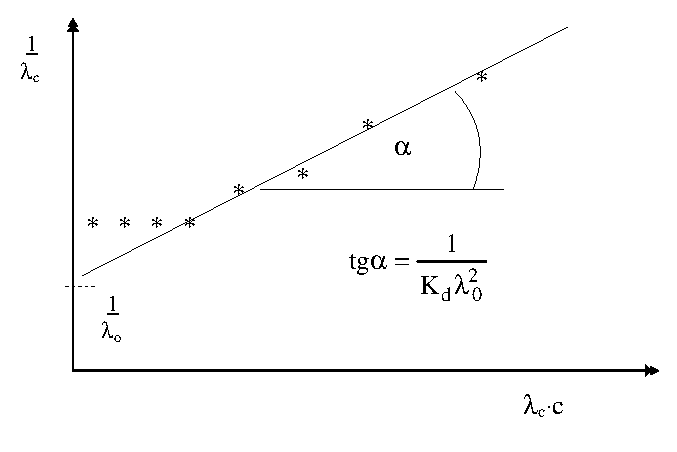
\includegraphics{fig/lambda0.eps}
\caption{Obtaining the limiting molar conductivity ($\lambda_0$).}
\label{fig:}
\end{figure}

\subsection{Practice procedures}

Rinse the electrode of the conductometer several times (4 - 5) with deionized water, the with ultrapure water ($\kappa$ < 1 $\upmu$S/cm). Ask the technician for ultrapure deionized water.

Prepare 20 v/v\% solution from an alcohol selected by the instructor. Then prepare two weak acid solutions (the weak acid is also selected by the instructor), from the stock solution (1 mol$\cdot$dm$^{-3}$) by pipetting 2.00 cm$^3$ into two 100 cm$^3$ measuring flasks, and then filling one with the 20 v/v\% alcohol solution, the other with ultrapure deionized water up to 100 cm$^3$.

Carry out the conductivity measurements in a measuring cilinder. Pour the water based solution into the cilinder and measure its conductivity. Then, pipette 25 cm$^3$ from the cilinder into a clean 50 cm$^3$ measuring flask, fill it up with ultrapure deionized water (2$\times$ dilution), and measure the conductivity of the new solution after carefully rinsing it with ultrapure deionized water. Repeat the dilution and measurement 3 times. Then do the same with the alcohol based solution, but using the 20 v/v\% alcohol solution for the dilutions and rinsing.

Note and record the temperature measured by the built-in thermometer of the electrode for each measurement.

Finally, measure the conductivity of the solvents as well (for the correction).
Then, to obtain the cell constant, measure the conductivity of 0.01 M KCl solution, and write down the temperature as well. Based on table 

Figure \ref{fig:vez} shows the schematics of a conductometric cell. A well-defined, inert electrode pair is submersed into an electrolyte, and the voltage drop between them is measured. Alternating current is used to avoid polarization and electrolysis.

\begin{figure}
\centering
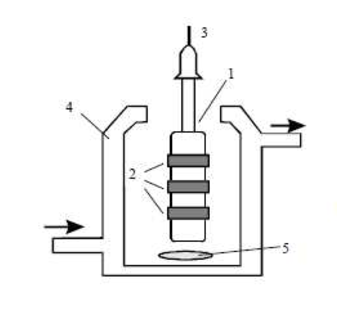
\includegraphics{fig/cond.eps}
\caption{Schematics of a conductometric cell. 1 - ,,bell electrode'', 2 - platinized platinum rings, 3 - electrical connection, 4 - double walled vessel, 5 - magnetic stirrer.}
\label{fig:vez}
\end{figure}

\subsection{Evaluation}

\begin{enumerate}
\item Calculate the cell constant.
Present the recorded data in such a table:

\begin{table}[!h]
\centering
\begin{tabular}{|c|c|c|c|c|c|c|c|}
\hline
c (mol $\cdot$ dm$^{-3}$) & G$_{\text{measured}}$ & $\kappa_{\text{korr}}$ (S $\cdot$ cm$^{-1}$) & $\lambda_c$ & $1/\lambda_c$ & $\lambda_c c$ & $\alpha$ & $K_d$ \\
\hline
... & ... & ... & ... & ... & ... & ... & ... \\
\end{tabular}
\label{table:vez}
\end{table}

\item Determine $\lambda_0$ graphically. Knowing $\lambda_c$ and $\lambda_0$, calculate $\alpha$ and $K_d$ for each concentration.

\end{enumerate}



\newpage
\section*{Appendix A -- Ionic conductivity at infinite dilution}
\addcontentsline{toc}{section}{Appendix B -- Ionic conductivity at infinite dilution}
The following table includes the molar ionic conductivities at infinite dilution for certain ions, that are necessary for evaluations in certain practices. The values refer to aqueous solutions at 25 $\celsius$.

\begin{table}[h!]
\centering
\caption{Molar ionic conductivity at infinite dilution. Source: CRC Handbook of Chemistry and Physics 76th edition, David R. Lide editor in chief, 1995-1996 ISBN: 0-8493-0476-8.}
\label{table:conductivities}
\vspace{5mm}
\begin{tabular}{l|c}
%\hline
                        Ion \hspace{2cm} & $\lambda^0_\pm$, $\cdot$10$^{-4}\cdot$m$^2 \cdot$S$\cdot$mol$^{-1}$\\
                      \hline


Ag$^+$ \dotfill & 61.9 \\
1/3 Al$^{3+}$ \dotfill& 61 \\
1/2 Ba$^{2+}$\dotfill& 63.6 \\
1/2 Be$^{2+}$\dotfill& 45 \\
1/2 Ca$^{2+}$\dotfill& 59.47 \\
1/2 Cd$^{2+}$\dotfill& 54 \\
1/3 Ce$^{3+}$\dotfill& 69.8 \\
1/2 Co$^{2+}$\dotfill& 55 \\
%1/3 [Co(NH$_3$)$_6$]$^{3+}$\dotfill& \\
%1/3 [Co(en)$_3$]$^{3+}$\dotfill& \\
%1/6 [Co$_2$(trien)$_3$]$^{6+}$\dotfill& \\
%1/3 Cr$^{3+}$\dotfill& \\
%Cs$^+$\dotfill& \\
1/2 Cu$^{2+}$\dotfill& 69.3 \\
%D$^+$\dotfill& \\
%1/3 Dy$^{3+}$\dotfill& \\
%1/3 Er$^{3+}$\dotfill& \\
%1/3 Eu$^{3+}$\dotfill& \\
1/2 Fe$^{2+}$\dotfill& 54 \\
1/3 Fe$^{3+}$\dotfill& 68 \\
%1/3 Gd$^{3+}$\dotfill& \\
H$^+$\dotfill& 67.3 \\
1/2 Hg$^{2+}$\dotfill& 68.6 \\
%1/2 Hg$^{2+}$\dotfill& \\
%1/3 Ho$^{3+}$\dotfill& \\
K$^+$\dotfill& 73.48 \\
%1/3 La$^{3+}$\dotfill& \\
%Li$^+$\dotfill& \\
1/2 Mg$^{2+}$\dotfill& 53.0 \\
%1/2 Mn$^{2+}$\dotfill& \\
%NH$_4^{+}$\dotfill& \\
%N$_2$H$_5^+$\dotfill& \\
1/2 CO$_3^{2-}$\dotfill & 69.3 \\

\end{tabular}
\end{table}


\end{document}
